\section{KẾT QUẢ ĐO VÀ ĐÁNH GIÁ}\label{sec:ket_qua}

\subsection{Failover link WAN tại Site 200}

Cắt uplink của vEdge 1 Site 200 trong khi ping liên tục qua overlay tới Campus chính, hai lần ngày 24/10/2026:

\begin{table}[H]
    \centering
    \small
    \caption{Kết quả failover link WAN vEdge 1 Site 200 (24/10/2026)}
    \label{tab:failover_s200}
    \begin{tabularx}{\textwidth}{|X|P{2.4cm}|P{2.4cm}|P{2.4cm}|}
        \hline
        \textbf{Chỉ số} & \textbf{Nhỏ nhất} & \textbf{Trung bình} & \textbf{Lớn nhất} \\
        \hline
        Thời gian khôi phục (RTO) & 7,68~s & 7,96~s & 8,25~s \\
        \hline
        Tỉ lệ khôi phục gói (PRR) & \multicolumn{3}{c|}{76,75\% (trung bình 2 lần)} \\
        \hline
    \end{tabularx}
\end{table}

\begin{figure}[H]
    \centering
    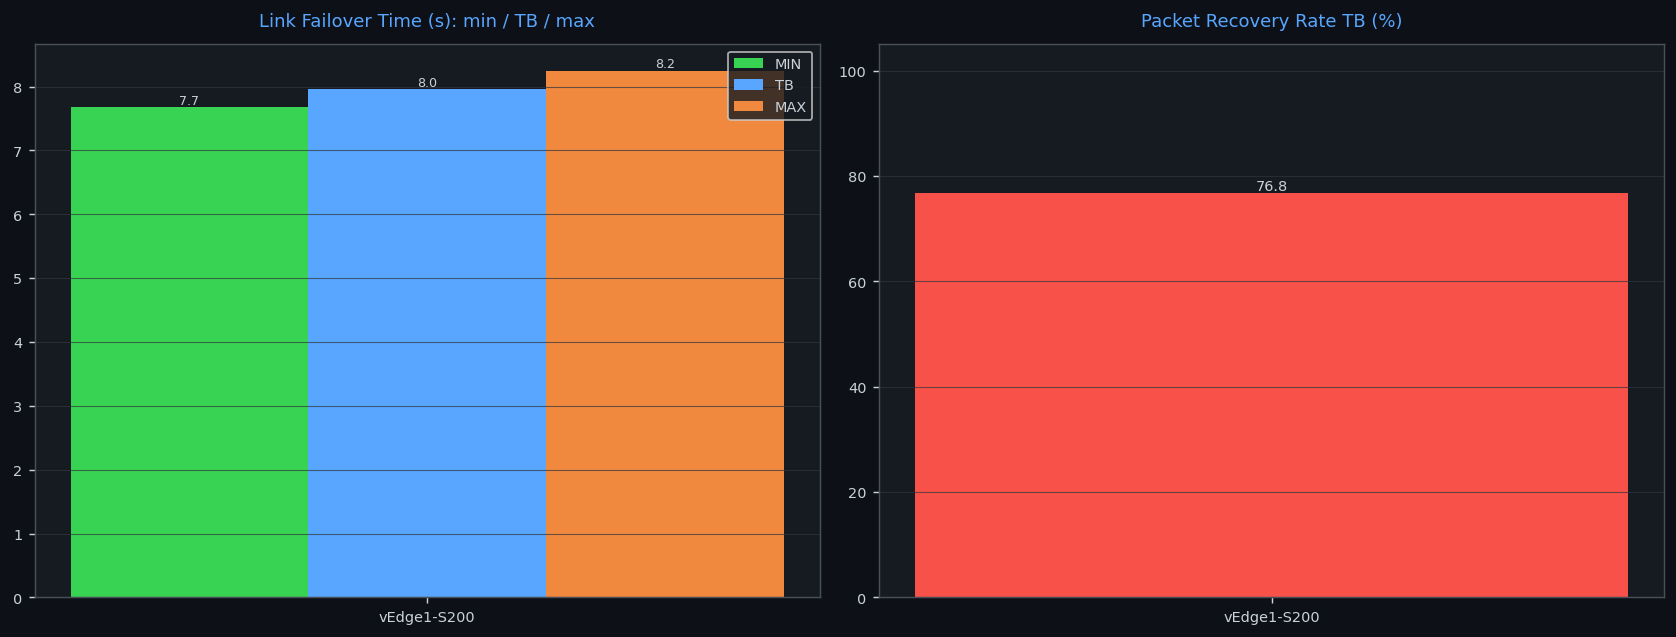
\includegraphics[width=0.9\linewidth]{image/tincay_failover.png}
    \caption{RTO và PRR khi cắt uplink vEdge 1 Site 200}
    \label{fig:tincay_failover}
\end{figure}

RTO khoảng 8~s phù hợp với tham số BFD mặc định của Viptela (hello 1~s, hệ số 7): phải mất khoảng 7~s để BFD kết luận tunnel chết rồi lưu lượng mới chuyển sang tunnel còn lại. Mới có hai lần đo nên chưa đủ để kết luận; tuần tới sẽ đo đủ 3--5 lần và thử giảm chu kỳ BFD để so sánh.

\subsection{So sánh hiệu năng Campus chính và chi nhánh}

Đo từ vEdge 1 của mỗi site tới các máy trạm trong site (LAN) và tới máy trạm, Web Server ở site khác qua SD-WAN (WAN), ngày 25/10/2026:

\begin{table}[H]
    \centering
    \small
    \caption{Delay, jitter và mất gói theo site (25/10/2026)}
    \label{tab:so_sanh}
    \begin{tabularx}{\textwidth}{|X|P{1.6cm}|P{1.6cm}|P{1.6cm}|P{1.6cm}|P{1.6cm}|}
        \hline
        \textbf{Site} & \textbf{Delay LAN (ms)} & \textbf{Delay WAN (ms)} & \textbf{Jitter WAN (ms)} & \textbf{Mất gói WAN} & \textbf{Tuyến LAN đo được} \\
        \hline
        Site 100 -- Campus chính & 6,26 & 4,00 & 0,53 & 0\% & 3/5 \\
        \hline
        Site 200 -- Cần Thơ & 2,83 & 7,56 & 5,09 & 0\% & 2/2 \\
        \hline
        Site 300 -- Đà Nẵng & 2,95 & 3,80 & 0,40 & 0\% & 2/2 \\
        \hline
        Site 400 -- Nha Trang & 4,30 & 11,96 & 10,33 & 0\% & 2/2 \\
        \hline
    \end{tabularx}
\end{table}

\begin{figure}[H]
    \centering
    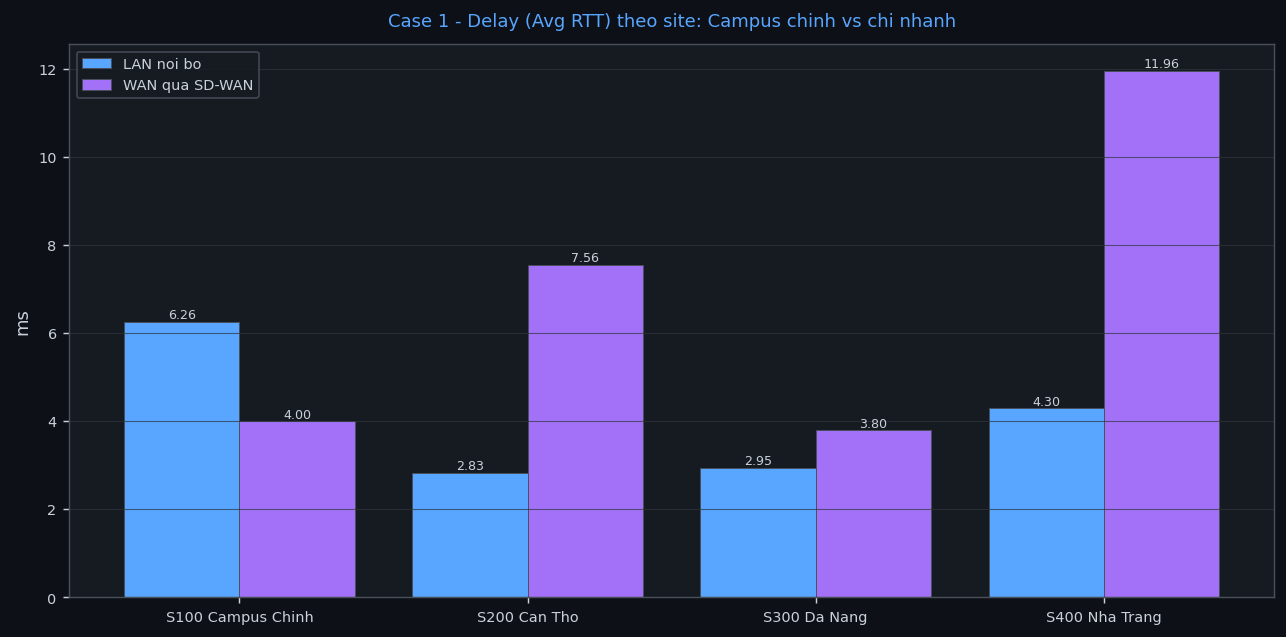
\includegraphics[width=0.9\linewidth]{image/sosanh_delay.png}
    \caption{Delay trung bình LAN và WAN theo site}
    \label{fig:sosanh_delay}
\end{figure}

\textbf{Nhận xét:}
\begin{itemize}
    \item Đường WAN qua SD-WAN \textbf{không mất gói} ở cả bốn site; delay WAN 3,8--12~ms.
    \item Site 400 có delay và jitter WAN cao nhất (12~ms, 10,3~ms), kế đến Site 200 (jitter 5,1~ms). Nguyên nhân là một vài mẫu RTT vọt lên 25--50~ms; cần đo lặp để xem có phải do tải máy ảo hay do đường đi.
    \item Site 100 chỉ đo được 3/5 tuyến LAN: hai tuyến từ vEdge Site 100 tới Web Server và DHCP-Server mất hết gói. Nhiều khả năng do chính sách firewall Site 100 chặn ICMP từ vùng SD-WAN vào Server Farm/DMZ (đúng thiết kế), nên cần đổi cách đo (dùng nguồn được phép hoặc đo TCP) thay vì coi là lỗi mạng.
\end{itemize}

\subsection{Đo lại sau khi thêm Site 500 (31/10/2026)}

Site 500 được dựng lại theo mô hình của các chi nhánh: vEdge 1 đi MPLS, vEdge 2 đi Internet, cả hai nối vào Brand-FW-S500 (ASAv), sau đó tới SW-S500 và máy trạm (VLAN 10, \texttt{10.5.10.0/24}). Công cụ đo được bổ sung Site 500: hai tuyến LAN (VPC11, PC Linux) và hai tuyến WAN (máy trạm và Web Server ở Campus chính), cộng thêm tuyến từ Campus chính tới VPC11.

Lần đo đầu tiên (14:56) cho thấy Site 500 chậm bất thường: delay LAN 18,6~ms trong khi các chi nhánh khác chỉ 3--4~ms. Ping từ vEdge tới Brand-FW của chính site cho thấy nguyên nhân nằm ở \textbf{số vCPU của vEdge}, không phải ở card mạng:

\begin{table}[H]
    \centering
    \small
    \caption{RTT từ vEdge tới Brand-FW cùng site theo cấu hình máy ảo (20 gói, 31/10/2026)}
    \label{tab:vcpu}
    \begin{tabularx}{\textwidth}{|X|P{1.6cm}|P{2.6cm}|P{2.6cm}|}
        \hline
        \textbf{vEdge} & \textbf{vCPU} & \textbf{Card mạng} & \textbf{RTT trung bình} \\
        \hline
        vEdge 1 Site 200 (mốc so sánh) & 2 & virtio & 0,80~ms \\
        \hline
        vEdge 2 Site 200 & 1 & virtio & 18,0~ms \\
        \hline
        vEdge 1 Site 500 -- trước & 1 & virtio & 17,0~ms \\
        \hline
        vEdge 2 Site 500 -- trước & 1 & e1000 & 16,6~ms \\
        \hline
        vEdge 1 Site 500 -- sau & 2 & virtio & 1,15~ms \\
        \hline
        vEdge 2 Site 500 -- sau & 2 & virtio & 0,99~ms \\
        \hline
    \end{tabularx}
\end{table}

vEdge chia vCPU thành lõi điều khiển và lõi chuyển tiếp dữ liệu (\texttt{show system status}: \textit{2 total, 1 control, 1 data}). Khi chỉ có 1 vCPU, hai việc này dùng chung một lõi nên mỗi gói qua vEdge chậm thêm khoảng 16~ms. Sau khi nâng hai vEdge Site 500 lên 2 vCPU, nhóm đo lại toàn bộ:

\begin{table}[H]
    \centering
    \small
    \caption{Delay, jitter và mất gói theo site sau khi thêm Site 500 (31/10/2026, 16:04)}
    \label{tab:so_sanh_3110}
    \begin{tabularx}{\textwidth}{|X|P{1.6cm}|P{1.6cm}|P{1.6cm}|P{1.6cm}|P{1.6cm}|}
        \hline
        \textbf{Site} & \textbf{Delay LAN (ms)} & \textbf{Delay WAN (ms)} & \textbf{Jitter WAN (ms)} & \textbf{Mất gói WAN} & \textbf{Tuyến LAN đo được} \\
        \hline
        Site 100 -- Campus chính & 9,99 & 4,12 & 0,76 & 0\% & 2/5 \\
        \hline
        Site 200 -- Cần Thơ & 3,64 & 5,85 & 2,19 & 0\% & 2/2 \\
        \hline
        Site 300 -- Đà Nẵng & 4,10 & 12,42 & 12,06 & 0\% & 2/2 \\
        \hline
        Site 400 -- Nha Trang & 4,24 & 9,58 & 7,16 & 0\% & 2/2 \\
        \hline
        Site 500 -- Campus Test & 3,02 & 10,46 & 4,18 & 0\% & 2/2 \\
        \hline
    \end{tabularx}
\end{table}

\begin{figure}[H]
    \centering
    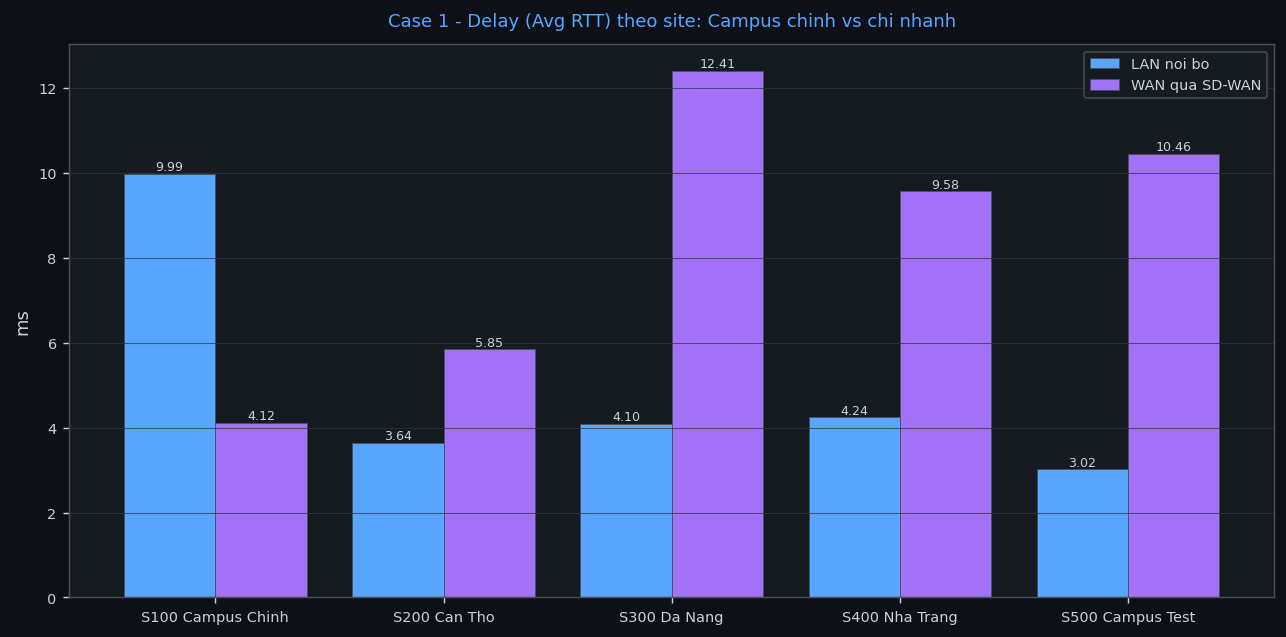
\includegraphics[width=0.9\linewidth]{image/sosanh_delay_3110.png}
    \caption{Delay trung bình LAN và WAN theo site, gồm Site 500 (31/10/2026)}
    \label{fig:sosanh_delay_3110}
\end{figure}

\textbf{Nhận xét:}
\begin{itemize}
    \item Sau khi nâng vCPU, Site 500 \textbf{ngang các chi nhánh khác}: delay LAN 18,6 $\rightarrow$ 3,0~ms; tuyến từ Campus chính tới VPC11 giảm từ 35,5 xuống 2,5~ms. WAN của cả năm site không mất gói.
    \item vEdge 2 của các site 100--400 vẫn đang chạy 1 vCPU, nên đường đi qua vEdge 2 (ví dụ khi failover sang Internet) có thể chậm thêm khoảng 16~ms. Cần nâng cấu hình trước khi đo failover để số liệu không bị sai lệch.
    \item Delay WAN của Site 300 và Site 400 (9,6--12,4~ms) và jitter cao chủ yếu do vài mẫu RTT vọt lên 29--46~ms; mỗi tuyến chỉ có ít mẫu nên một mẫu chậm (máy chủ EVE đang tải cao) cũng làm trung bình tăng. Cần đo lặp 2--3 lần và lấy trung bình cho báo cáo cuối kỳ.
    \item Site 100 chỉ đo được 2/5 tuyến LAN: ngoài Web Server và DHCP-Server, lần này tuyến tới máy trạm PC-Luat-S100-1 (VLAN 30) cũng mất hết gói. Tuyến này không đi qua Server Farm/DMZ nên không giải thích được bằng chính sách firewall; cần kiểm tra riêng sau khi chuyển firewall Site 100 sang HA kiểu doanh nghiệp.
\end{itemize}

\subsection{Kiểm thử tích hợp}

\begin{table}[H]
    \centering
    \small
    \caption{Kết quả kiểm thử tích hợp toàn hệ thống (25/10/2026)}
    \label{tab:tich_hop}
    \begin{tabularx}{\textwidth}{|P{3.6cm}|X|P{1.6cm}|}
        \hline
        \textbf{Cụm} & \textbf{Kết quả} & \textbf{Đánh giá} \\
        \hline
        SDN Site 100 & 6/6 OVS, 13/13 liên kết; 7/7 máy trạm nhận DHCP, thông liên VLAN & ĐẠT \\
        \hline
        Firewall HA & Active / Standby Ready & ĐẠT \\
        \hline
        SD-WAN & 12/12 thiết bị reachable, BFD 92/92 & ĐẠT \\
        \hline
        Chi nhánh 200/300/400 & 9/9 VPC + 3 PC Linux nhận DHCP; tới Web/Mail/DNS Site 100 (TCP 80, 443, 25, 143, 587) & ĐẠT \\
        \hline
        Internet & 4/4 site ra Internet (sau khi sửa bộ lọc BGP Site 500) & ĐẠT \\
        \hline
        Quản trị in-band chi nhánh (30/10) & Ping 15/15 địa chỉ quản trị; SSH 12/12 thiết bị & ĐẠT \\
        \hline
    \end{tabularx}
\end{table}

\subsection{Đánh giá}

\begin{itemize}
    \item Hệ thống chạy đồng thời đủ các cụm và đạt toàn bộ kiểm thử chức năng; đây là nền để chuyển sang kiểm thử sự cố (failover firewall, cắt một màu WAN) trong tuần tới.
    \item Số liệu SD-WAN mới là bước đầu: RTO khoảng 8~s và PRR 76,75\% cho thấy failover dựa vào BFD mặc định khá chậm so với SDN (fast-failover dưới 0,3~s). Đây là điểm sẽ phân tích trong báo cáo cuối kỳ.
    \item NetOps Bot đã chẩn đoán đúng một lệch thiết kế có thật: uplink của hai switch phòng ban Site 400 đang lên trunk nhờ DTP tự thỏa thuận chứ không cấu hình tường minh. Lỗi này được giữ lại để làm kịch bản demo ``phát hiện -- sửa bằng \texttt{/change} -- tự rollback''.
\end{itemize}
